\section[Využití synchrotronového záření v materiálovém výzkumu]{Využití synchrotronového záření v materiálovém výzkumu: získávání synchrotronového záření a jeho vlastnosti, příklady experimentálních technik}

Synchrotronové záření, někdy také nazývané jako magnetické brzdné záření, je záření vysílané relativistickými elektrony kroužícími v magnetickém poli a vzniká tak při pohybu nabité částice se zrychlením. Dochází tak k uvolňování EM záření. Jelikož je zrychlení vektorové, nemusí docházet ke zpomalování nebo zrychlování nabité částice, ale stačí změna dráhy pohybu a tím se také utváří zrychlení, jež vede na uvolnění části energie do okolí.

Dále platí, že pokud je při změně dráhy pohybu rychlost částice malá, tak emitované záření je uvolňováno izotropně. Pokud je rychlost vysoká (v/c je cca 1), tak je záření soustředěno do kuželu ve směru pohybu částice s určitým úhlem rozevření kužele, jež závisí na Lorentzovu faktoru, který je nepřímo úměrný rychlosti (čím větší rychlost tím menší rozevření kužele).

\subsection{Schéma uspořádání synchrotronu}

Sychrotron je cyklický urychlovač částic, jež se skládá z elektronového děla, lineárního urychlovače pro prvotní zrychlení částice a posléze ze dvou prstenců (urychlující a akumulační). Vývodem akumulačního prstence je trasa vedoucí do koncové stanice, kde je realizován experiemnt.

\begin{figure}[H]
	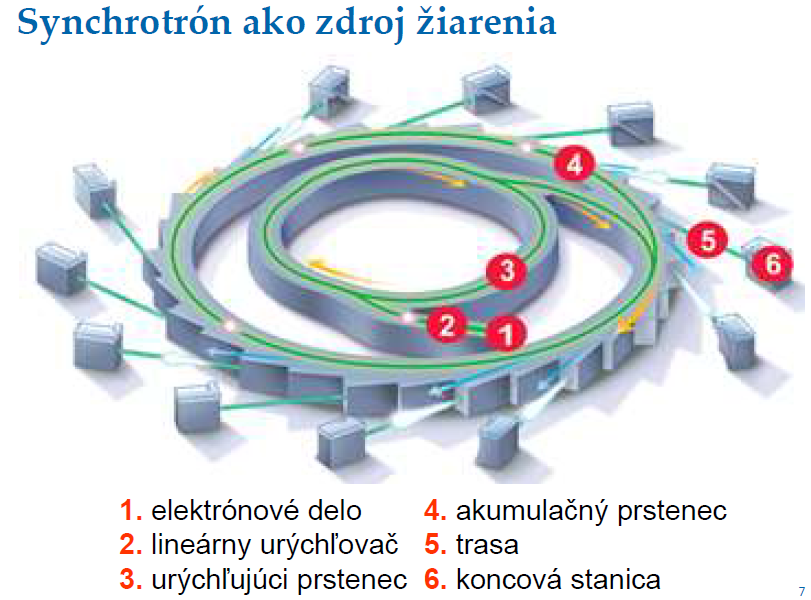
\includegraphics[width=7cm]{img/synchrotron.png}
	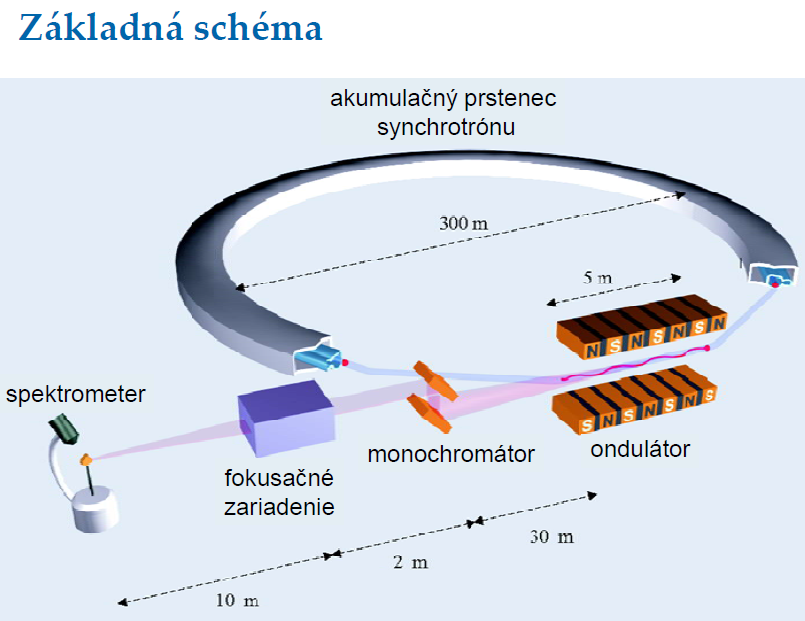
\includegraphics[width=7cm]{img/synchrotron2.png}
\end{figure}

\subsection{Tvorba synchrotronového záření}

Bylo již řečeno v jakých případech a jak vzniká synchrotronové záření, ale jak se to dělá v praxi? V praxi se využívá tzv. vkládacích zařízení, kterými jsou: ohybací magnet (bending magnet), Wigglery a Ondulátory.

\begin{itemize}
    \item \textbf{Ohybací magnet}: slouží k zakřivení dráhy pohybu nabité částice a přitom je tečně k dráze pohybu uvolňováno záření, které se pak dá kolimovat.

    \begin{figure}[H]
        \centering
        \includegraphics[width=0.5\linewidth]{img/ohybací magnet.png}
        \caption{ohybací magnet}
    \end{figure}

    \item \textbf{Wiggler}: zařízení, jež je tvořeno větším počtem dvojic permanentních magnetů, které zapříčiní klikacení dráhy pohybu částice a to způsobuje tvorbu širokého svazku nekoherentního záření. Intenzita záření je úměrná N (počet magnetů).

    \begin{figure}[H]
        \centering
        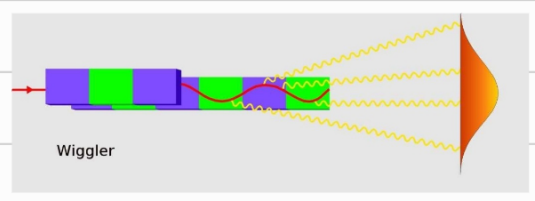
\includegraphics[width=0.5\linewidth]{img/Wiggler.png}
        \caption{Wiggler}
    \end{figure}
        
    \item \textbf{Ondulátor}: je to to samé co wiggler (opět permanentní magnety), ale magnety jsou slabé a je to asi i delší. Ta částice se tudíž neklikatí tolik a výsledná intenzita emitovaného záření je dokonce úměrná $N^2$, kde N je počet magnetů

    \begin{figure}[H]
        \centering
        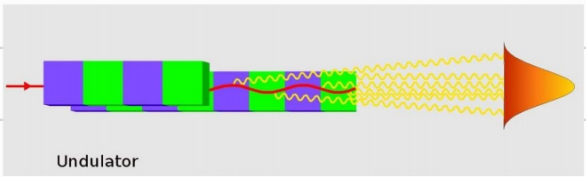
\includegraphics[width=0.5\linewidth]{img/Ondulátor.png}
        \caption{Ondulátor}
    \end{figure}
\end{itemize}

\subsection{Vlastnosti synchrotronového záření}

\begin{itemize}
    \item Spojité a velmi široké spektrum (od IR po RTG záření).
    \item Vysoká monochromatizace.
    \item Při využití ondulátorů, je záření koherentní.
    \item Stabilita svazku.
    \item Impulzní emise (záření je emitované časticemi a podle počtu částic je to víc spojité a nebo více impulsní).
    \item Přeladitelnost (můžeme si vybrat energii) $\rightarrow$ více stupňová monochromatizace na monokrystalech Si $\rightarrow$ Monochromátor s vysokým rozlišením (rozptyl cca 1 meV) $\rightarrow$ kolimace a fokusace pomocí Be čočky nebo K-B zrcadlo a tím fokusace až na rozměry 4x10 $\mu m^2$.
    \item Polarizované.
    \item Briliance = kombinace toku, velikost zdroje, divergence svazku = jedná se v zásadě o trochu komplikovanější Intenzitu pro popis elektromagnetického záření. 
\end{itemize}

\textbf{Využití}

\begin{itemize}
    \item Dá se využít pro jaderný rezonanční rozptyl (studium hyperjemných interakcí, vibrační vlastnosti jader, magnetické přechody apod., a to za extrémních vnějších podmínek = magnetické pole, kryo, vysoká teplota apod..).
    \item RTG mikroskopie -- využití RTG svazků s rozlišením v řádu desítek nm a zobrazení tenkých vrstev a povrchů.
    \item Transmisní X-ray mikroskopie (TXM) -- Dobrý kontrast, vysoké rozlišení.
    \item RTG sepktroskopie = měření chemického složení.
    \item RTG absorpční spektroskopie = informace o typu a vzdálenostech sousedních atomů.
    \item RTG tomografie = 3D obrazy drobných objektů s velmi vysokým rozlišením na úrovni mikrometrů.
\end{itemize}

\subsection{XFEL} 

Zařízení XFEL (X-Ray Free Electron Laser) je zařízení, které je v podobě lineárního urychlovače (European XFEL, SwissFEL) a umožňuje lineárně urychlovat elektrony až na energie 17 GeV. Urychlené elektrony pak projdou ondulátorem a vzníká záření jako ze synchrotronu, které má rozsah energií od 0,01 - 20 keV (velmi malá vlnová délka).

$\rightarrow$ Velmi malá krátkost pulsů (cca desítky fs)

$\rightarrow$ O 10 řádů vyšší briliance jako u 3. generace sychrotronů. 

$\rightarrow$ V zásadě jsou dány frekvence na balík (jak často přichází balík elektronů, resp. pulsu), ale pak je ještě samotná frekvence v rámci balíku a proto je krátkost pulsů velmi malá.

\begin{figure}[H]
    \centering
    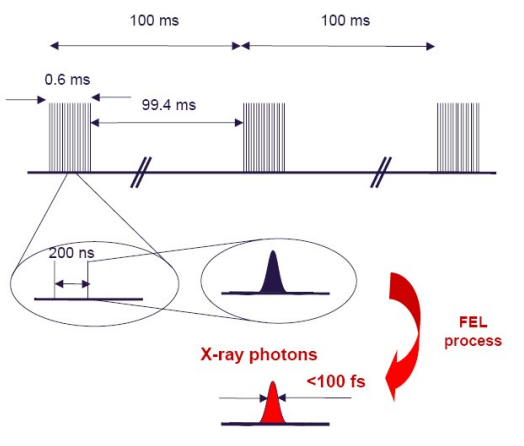
\includegraphics[width=0.5\linewidth]{img/časová struktura pulsů fotonů.png}
    \caption{časová struktura pulsů fotonů}
\end{figure}

\newpage
\mbox{}
\newpage
